\newpage
\appendix
\section{Appendix}

\subsection{Proof of consistency theorem}
\label{appendix:theorem_proof}

Proof of the theorem in \ref{sec:theorem}:

\begin{theorem*}[B2B consistency - general case]

     Consider the B2B model from Equation $Y = (XE + N)F$, $N$ centred and full rank noise.
     %
     If $F$ and $X$ are full-rank on $Img(E)$, then, the solution of B2B, $\hat H$, will minimize
     %
     $\min_H  \left \| X - XH\right\| ^2  + \left \| NH\right \| ^2$and satisfy $E\hat H = \hat H$
\end{theorem*}

\begin{proof}

 Let $\hat G$ and $\hat H$ be the solutions of the first and second regressions of B2B, we have
 \begin{align*}
    \hat G = \arg \min_G \mathbb{E}[\left \| YG - X \right \|^2] &=   \arg \min_G \mathbb{E}[\left \| X - (XE + N)FG \right\|^2]\\
%                                                        &{}= \arg \min_G \mathbb{E}[\left \| X - XEFG\right\| ^2]  + \mathbb{E}[\left \| NFG\right \| ^2]\\
                                                        &{}= \arg \min_G \left \| X - XEFG\right\| ^2  + \left \| NFG\right \| ^2
     \label{eq:doublenorm}
\end{align*}
\begin{align*}
    \hat H = \arg \min_H \mathbb{E}[\| XH - Y \hat{G} \|^2] &=\arg  \min_H \mathbb{E}[\| XH - (XE + N)F \hat G \|^2] \\
    &=\arg \min_H \mathbb{E}[\| X(H - EF \hat G) \| ^2] + \mathbb{E}[\| NF\hat G \| ^2]\\
%    &= \arg \min_H \mathbb{E}[\| X(H - EF \hat G) \| ^2]\\
    &= EF \hat G
\end{align*}

Let us prove that $EF\hat G = F\hat G$, that is, that the $d_x$ bottom rows of $F\hat G$ are zero. Let $Z=F^\dagger EF\hat G$. We have $FZ = FF^\dagger EF  \hat G= EF\hat G$ ($FF^\dagger E =E$ since $F$ is full rank on $Img(E)$). Since E is a contraction, we have $ \| NEF\hat G\|^2 \leq \| NF\hat G \|^2$. Therefore,
 $$\left \| X - XEFZ\right \| ^2  + \left \| NFZ\right \| ^2 = \| X - XEF\hat G \| ^2  + \| NEF\hat G \| ^2 \leq \| X - XEF\hat G \| ^2  + \| NF\hat G \| ^2$$

But as $\hat G =  \arg \min_G \left \| X - XEFG\right\| ^2  + \left \| NFG\right \| ^2$, the above inequality is an equality, $Z=\hat G$ and $EF\hat G = F\Hat G$. Therefore, $\left \| X - XEFG\right \| ^2  + \left \| NFG\right \| ^2 = \left \| X - XEFG\right \| ^2  + \left \| NEFG\right \| ^2 = \left \| X - XH\right \| ^2  + \left \| NH\right \| ^2$ is minimised by $\hat G$ and $\hat H$. Finally, $E\hat H = E EF\hat G = EF\hat G = \hat H$. This completes the proof.
\end{proof}

\newpage
\subsection{Feature importance}
\label{appendix:feature_importance}

For B2B, feature importance is assessed as follows:

\begin{algorithm}[H]
    %\SetAlgoLined
    \KwIn{$X_{train} \in \mathbb{R}^{n \times d_x}$, $X_{test} \in
\mathbb{R}^{n' \times d_x}$, $Y_{train} \in \mathbb{R}^{n\times d_y}$, $Y_{test}
\in \mathbb{R}^{n'\times d_y}$, } \KwOut{estimate of prediction improvement
$\Delta{R} \in \mathbb{D}^{d_x}$.} $H, G = \text{B2B}(X_{train}, Y_{train})$\;
$R_{full} = \text{corr}(X_{test} H, Y_{test} G)$\;

    \For{$i = 1, \ldots, d_x$}{ $K = Id$\; $K[i] \leftarrow 0$\; $H_k =
\text{LinearRegression}(X_{train} K, Y_{train} G_i)$\; $R_{k} =
\text{corr}(X_{test} H_k, Y_{test} G_i)$\; $\Delta R_i = R_{full} - R_{k}$\; }
\Return{$\Delta R$} \caption{B2B feature importance.} \label{algorithm:b2b_fi}
\end{algorithm}

For the Forward Model, the feature importance is assessed as follows:

\begin{algorithm}[H]
    %\SetAlgoLined
    \KwIn{$X_{train} \in \mathbb{R}^{n \times d_x}$, $X_{test} \in
\mathbb{R}^{n' \times d_x}$, $Y_{train} \in \mathbb{R}^{n\times d_y}$, $Y_{test}
\in \mathbb{R}^{n'\times d_y}$, } \KwOut{estimate of prediction improvement
$\Delta{R} \in \mathbb{D}^{d_x, d_y}$.} $H = \text{LinearRegression}(X_{train},
Y_{train})$\; $R_{full} = \text{corr}(X_{test} H, Y_{test})$\;

    \For{$i = 1, \ldots, d_x$}{ $K = Id$\; $K[i] \leftarrow 0$\; $H_k =
\text{LinearRegression}(X_{train} K, Y_{train})$\; $R_{k} = \text{corr}(X_{test}
{H_k}, Y_{test})$\; $\Delta R_i = R_{full} - R_{k}$\; } \Return{$\Delta R$}
\caption{Forward feature importance.} \label{algorithm:fwd_fi} \end{algorithm}

% \iffalse
% \begin{enumerate}
%   \item Fit $H$ given $X_{train}$ and $Y_{train}$
%   \item For each feature $i$:
%   \begin{itemize}
%     \item Define $K$, and identity matrix whose row $i$ has been zeroed-out
%     \item Fit $H^i_k$ given $X_{train} K$ and $Y_{train}$
%   \end{itemize}
%   \end{enumerate}
% \fi

For the CCA and PLS models, the feature importance is assessed as follows:

\begin{algorithm}[H]
    %\SetAlgoLined
    \KwIn{$X_{train} \in \mathbb{R}^{n \times d_x}$, $X_{test} \in
\mathbb{R}^{n' \times d_x}$, $Y_{train} \in \mathbb{R}^{n\times d_y}$, $Y_{test}
\in \mathbb{R}^{n'\times d_y}$, } \KwOut{estimate of prediction improvement
$\Delta{R} \in \mathbb{D}^{d_x, d_z}$.} $H, G = \text{CCA}(X_{train},
Y_{train})$\; $R_{full} = \text{corr}(X_{test} H, Y_{test} G)$\;

    \For{$i = 1, \ldots, d_x$}{ $K = Id$\; $K[i] \leftarrow 0$\; $H_k, G_k =
\text{CCA}(X_{train} K, Y_{train})$\; $R_{k} = \text{corr}(X_{test} H_k,
Y_{test} G_k)$\; $\Delta R_i = R_{full} - R_{k}$\; } \Return{$\Delta R$}
\caption{CCA and PLS feature importance.} \label{algorithm:cdp_fi}
\end{algorithm}

For the Backward Model, feature importance cannot be assessed because there is no prediction.


\section{Additional Figures}


\begin{figure}[t!]
  \centering
  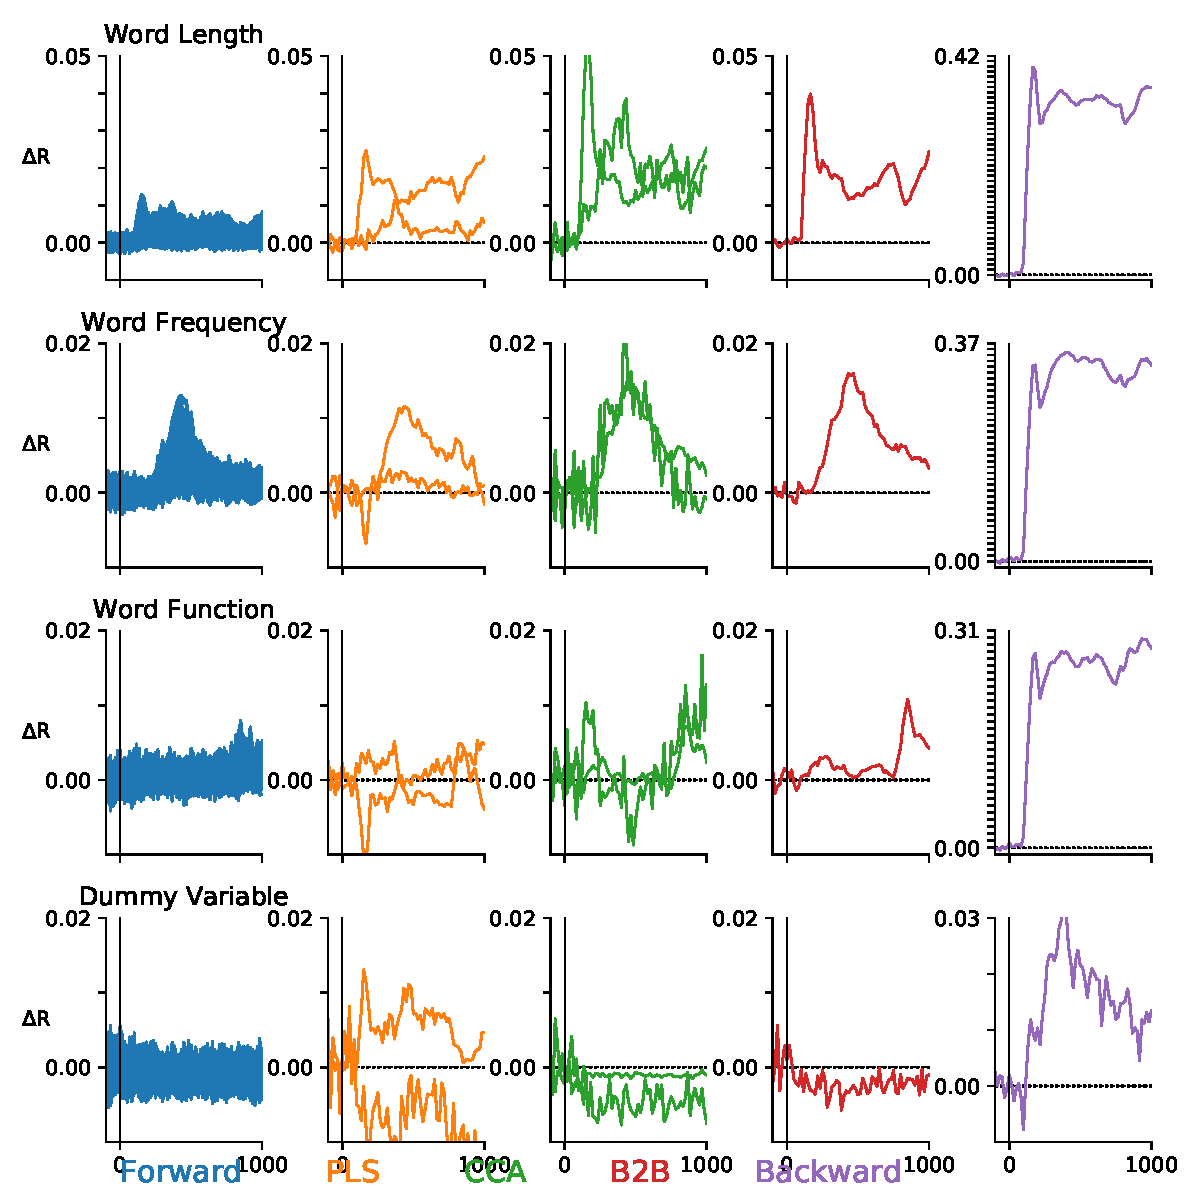
\includegraphics[width=\textwidth, trim=0cm 0cm 0cm 0cm, clip=True]{figures/meg_supp.pdf}
  \caption{}
  \label{fig:meg_supp}
\end{figure}


\begin{figure}
  \centering
  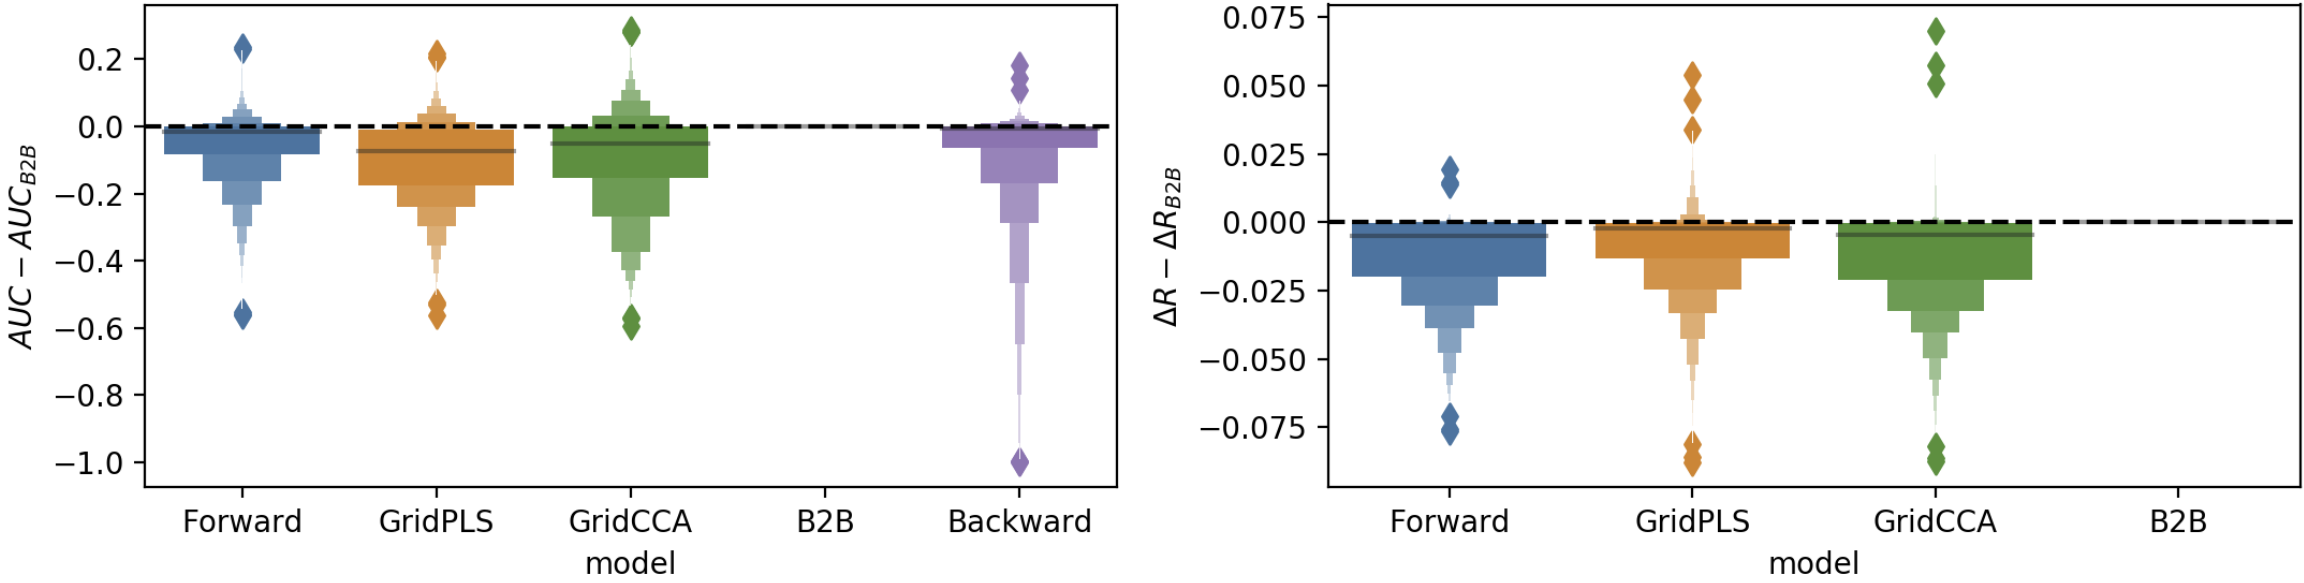
\includegraphics[width=\linewidth]{figures/AUC_R.png}
  \caption{Synthetic experiments. Distribution (over conditions) of differences in AUC (left) and Feature Importance $\Delta R$ (right) metrics between our method and the baselines. Mass under the dashed line corresponds to B2B outperforming the baseline. \label{fig:auc_plots}}
\end{figure}
